% ---------------------------------------------------------------------------
% Revised draft: A Representation-Centred Evaluation of Latent Diffusion for
% Afrikaans Text Generation (BSc Honours, Wits CSAM).
%
% Build in the TACL template folder (needs tacl2021v1.sty and acl_natbib.bst):
%   xelatex main && bibtex main && xelatex main && xelatex main
% pdfLaTeX also works.
%
% Conventions used in this file
%   \textbf{[XX: ...]}    result or fact still to be supplied; never estimate it
%   \textbf{[CITE: ...]}  suggested citation not yet verified; never cite as is
%   \textbf{[tool, version]} etc.  blanks for the author to fill in
%   E1--E12               experiments listed in the change log / placeholder list
% Search for "[XX:" and "[CITE:" before submission: neither may remain.
% ---------------------------------------------------------------------------
\documentclass[11pt,a4paper]{article}
\usepackage[acceptedWithA]{tacl2021v1}
\usepackage{iftex}
\ifPDFTeX
  \usepackage[utf8]{inputenc}
  \usepackage[T1]{fontenc}
\fi
\usepackage{times}
\usepackage{latexsym}
\usepackage{amsmath}
\usepackage{amssymb}
\usepackage{booktabs}
\usepackage{tabularx}
\usepackage{graphicx}
\usepackage{adjustbox}
\usepackage{url}
\usepackage{microtype}

\title{A Representation-Centred Evaluation of Latent Diffusion\\for Afrikaans Text Generation}

\author{Hadi Butt\\
School of Computer Science and Applied Mathematics\\
University of the Witwatersrand, Johannesburg}

\date{}

\begin{document}
\maketitle

% Abstract.
\begin{abstract}
Latent diffusion generates text by denoising in a continuous space and decoding the result, so every sample passes through the autoencoder that defines that space. We test what this means for unconditional Afrikaans generation on the NCHLT corpus, using an mT5-base encoder--decoder adapted with a Perceiver bottleneck and two diffusion denoisers trained with five seeds each. The autoencoder reproduces only 11 of 81 held-out passages exactly and keeps 21 of 33 numerals; shuffling latents across documents shows that the decoder uses the latent, not that the latent preserves the passage. Favourable generation scores coexist with this. The larger denoiser lowers external mGPT perplexity from 51.31 to 48.61, yet random latents decoded by the same decoder reach similar raw perplexity although only 5.5\% of their outputs are identified as Afrikaans, and a second Afrikaans scorer even prefers them to diffusion output. Retraining the decoder alone raises reconstruction chrF only from 67.70 to 70.05, but an autoencoder with all parameters trained reconstructs 73 of 103 reserve passages exactly, against 19 for the original. Favourable raw perplexity therefore did not establish reconstruction fidelity, which has to be measured alongside generation scores.
\end{abstract}

% ===========================================================================
\section{Introduction}
% ===========================================================================

A government notice states that the Departement van Maatskaplike Dienste en Armoedeverligting (Social Services and Poverty Alleviation) offers 44 bursaries a year, 20 of them for social development. Encoded into a latent and decoded again by an Afrikaans text autoencoder, the passage keeps 44, loses 20, and the department becomes ``Maatskaplike Ontwikkeling'' (Social Development). Latent text diffusion generates through such an autoencoder: a denoiser produces a latent, and a decoder turns it into words \citep{lovelace2023latent}. In unconditional generation there is no source passage to compare against, so scores on generated text cannot show whether the autoencoder preserves content. Reconstruction does not measure the quality of generated text; it tests whether the latent space represents passages faithfully, which a latent generator relies on to express specific content such as names and numbers.

Latent text diffusion has been evaluated mainly on English, by scoring generated text \citep{li2022diffusionlm,gong2023diffuseq,lovelace2023latent}. We found no study that tests whether its autoencoder preserves passages when adapted with limited in-domain data; \citet{lovelace2023latent} report reconstruction for English only. Afrikaans is an informative case: the NCHLT (National Centre for Human Language Technology) corpus offers licensed government-domain text \citep{eiselen2014developing} but only about 1.2 million training words, while Afrikaans is covered by a pretrained encoder--decoder, mT5 \citep{xue2021mt5}, and an external scorer, mGPT \citep{shliazhko2024mgpt}. We ask:
\begin{enumerate}
\item \textbf{RQ1:} What constraints does a reduced English reproduction of the pipeline identify before the Afrikaans results are interpreted?
\item \textbf{RQ2:} Do autoencoders adapted to NCHLT Afrikaans preserve enough of a passage for faithful reconstruction?
\item \textbf{RQ3:} Does Afrikaans latent diffusion compare credibly with an autoregressive (AR) baseline under mGPT perplexity, diversity and repetition diagnostics, and tokenisation fertility?
\end{enumerate}

Under criteria fixed in the research proposal before the experiments, the system is credible if its reconstructions preserve content, its mGPT perplexity is at most 1.20 times that of the AR baseline, and its outputs show no severe repetition or loss of diversity. The AR baseline shares corpus and tokeniser but is trained from scratch and sampled with nucleus sampling, whereas the diffusion system decodes with a pretrained decoder and beam search, so the comparison sets two systems against each other, not two generation mechanisms.

Our central finding is that favourable generation scores and unfaithful reconstruction coexist in the same system, and that favourable raw perplexity did not establish reconstruction fidelity. We contribute (i) a reconstruction analysis that separates use of the latent from preservation of the passage; (ii) evidence, from a random-latent control, language identification and a second scorer, that raw generation scores do not track this failure; and (iii) a follow-up autoencoder screen with rules fixed in advance, showing that the failure is not inherent to the setting.

% ===========================================================================
\section{Related work}
% ===========================================================================

Diffusion models generate by reversing a gradual noising process \citep{ho2020denoising,nichol2021improved}. For text, tokens have been handled by diffusing over discrete states \citep{austin2021structured}, over continuous embeddings \citep{li2022diffusionlm,gong2023diffuseq,strudel2022self,dieleman2022continuous}, or with likelihood-trained continuous models \citep{gulrajani2023likelihood}. Latent diffusion instead denoises in an autoencoder's latent space \citep{rombach2022high}; \citet{lovelace2023latent} apply this to language by compressing a pretrained encoder--decoder, and \citet{zhang2023planner} extend it to paragraphs. A latent model can generate only what its decoder can express: strong decoders may ignore their latent \citep{bowman2016generating,li2020optimus}, and bottleneck autoencoders trade compression against reconstruction \citep{montero2021sentence}.

Open-ended generation has no reference output, so it is usually scored with an external language model and diversity statistics. Probability and quality can disagree \citep{holtzman2020curious,meister2020beam}, which motivated distribution-level measures \citep{pillutla2021mauve}, and any metric needs validating for its use \citep{reiter2018structured}. Resources for African languages remain uneven \citep{joshi2020state,nekoto2020participatory}, although models pretrained on modest data can be competitive \citep{ogueji2021small,adebara2023serengeti} and Afrikaans-specific encoders exist \citep{ralethe2020adaptation}. We found no evaluation of diffusion-based generation for Afrikaans.

% ===========================================================================
\section{Data and method}
\label{sec:method}
% ===========================================================================

\paragraph{Corpus.} We use the clean 2.0 distribution of NCHLT Afrikaans (government-domain text, CC BY 2.5 South Africa) \citep{eiselen2014developing}. Text is NFC- and whitespace-normalised, contact details are masked, and passages of at most 50 words are formed; passages under three words and exact duplicates are removed, and no language-identification filter is applied. Documents are split with seed 42 into 47,767 training, 5,905 validation and 5,692 test passages (2,005, 251 and 251 documents); no passage is shared across splits, although some 12-word sequences are. We keep the mT5 tokeniser (250,100 entries, 128-token cap) instead of training a SentencePiece vocabulary \citep{kudo2018sentencepiece} as proposed, because the pretrained embeddings depend on it; validation fertility is 1.933 tokens per word.

\paragraph{Autoencoder and diffusion.} Following \citet{lovelace2023latent}, the mT5-base encoder feeds a three-layer Perceiver \citep{jaegle2021perceiver} that compresses its states to a latent of 32 slots (vectors) of dimension 64, each rescaled to norm eight, and a reconstruction map passes it to the mT5 decoder. Only the Perceiver components, the final decoder block and the final layer norm are trained, with teacher-forced cross-entropy (CE); we use update 30,500 (effective batch eight) of a run that continued an earlier pilot. Keeping the pretrained encoder and most of the decoder frozen follows the design adopted for the English reproduction; the follow-up screen (\S\ref{sec:res-aescreen}) trains every parameter instead. Denoisers are trained to predict the velocity \citep{salimans2022progressive} under a cosine schedule \citep{nichol2021improved}, with self-conditioning \citep{chen2023analog}. The code is a fork of the official implementation of \citet{lovelace2023latent}.

\paragraph{Systems.} The small and large denoisers (width/depth/heads 256/4/4 and 768/12/12; 8.1M and 188M parameters) are trained with seeds 42--46, selecting the checkpoint with the lowest velocity mean squared error of an exponential moving average (EMA) of the weights on a validation probe. Each run samples latents with 250 denoising diffusion probabilistic model (DDPM) steps \citep{ho2020denoising} and decodes them with beam search (four beams, repetition penalty 1.2, no repeated trigrams), producing 1,000 validation and 1,000 test samples. The AR baseline is a four-layer GPT-style model (width 256; 67M parameters, of which 64M, or 95\%, are its tied 250,100-entry embedding) trained from scratch on the same splits (Table~\ref{tab:conditions}); its checkpoint at update 60,000 is selected on validation CE, and it produces 256 validation samples with nucleus sampling ($p=0.95$, temperature one). Beam search is not used for AR, because from a fixed start token it returns the same output every time. As a decoder-only control, 1,000 Gaussian latents rescaled to norm eight are decoded with the same decoder (validation only).

\begin{table*}[t]
\centering
\small
\begin{adjustbox}{max width=\textwidth}
\begin{tabular}{llll}
\toprule
Condition & Small diffusion & Large diffusion & AR baseline \\
\midrule
Pretrained weights & Adapted mT5 & Same adapted mT5 & None (random initialisation) \\
Generator parameters & 8.10M & 187.98M & 67.22M \\
Training seeds & 42--46 & 42--46 & 42 \\
Precision / effective batch & FP32 / up to 64 & FP32 / up to 64 & BF16 / 8 \\
Exposure at selection & 288--306 epochs & 172--180 epochs & 480,000 sampled passages \\
Recorded training time & 2.93--3.13 h & 7.19--7.85 h & 4.52 h \\
Text decoding & Beam 4, constrained & Beam 4, constrained & Nucleus, $p=0.95$, temperature 1 \\
\bottomrule
\end{tabular}
\end{adjustbox}
\caption{Comparison conditions (RQ3). All systems use the same splits and tokeniser. Diffusion parameter counts exclude the shared autoencoder; the AR count includes its tied 250,100-entry embedding, so counts are not whole-system equivalents. Training times cover training and checkpoint selection on an RTX PRO 6000 Blackwell and exclude pretraining and autoencoder training. AR passages are sampled with replacement, so they are not complete epochs.}
\label{tab:conditions}
\end{table*}

% ===========================================================================
\section{Evaluation}
\label{sec:evaluation}
% ===========================================================================

\paragraph{Reconstruction.} On 81 validation passages from 64 documents we report teacher-forced CE and, for free-running output, exact matches, mean sentence chrF \citep{popovic2015chrf} and numeral recall and precision. As a control, each latent is replaced by that of a passage from another document of similar length. All 81 reconstructions were also labelled, as an exploratory reading, against three pre-specified content checks: named entities and content words preserved, main clause recognisable, and no unsupported material. The labels were produced by an AI assistant that saw each source beside its reconstruction; they were not verified by the author or an Afrikaans reader.

\paragraph{Generation.} All text is scored with mGPT (FP32, 512-token window, stride 256), each output separately after a start token. Perplexity (PPL) is token-weighted over a sample set and is not the generator's own likelihood. We also report mean length, distinct-2, exact training copies and the share of outputs identified as Afrikaans by GlotLID v3 \citep{kargaran2023glotlid}, with a dictionary check against the LibreOffice \texttt{af\_ZA} Hunspell list. Because mGPT is strongly length-dependent, comparisons are repeated with length-standardised perplexity, which reweights per-band log-loss (1--10, 11--20, 21--35 and 36+ words) to the human length distribution, and under a second scorer, the monolingual Afrikaans Goldfish model \citep{chang2024goldfish}. Goldfish's model card does not list NCHLT; one of its source collections, Glot500, includes NCHLT corpora, so overlap with our data cannot be ruled out.

\paragraph{Uncertainty and data use.} Diffusion values are means over five runs. The large-minus-small difference has a run bootstrap, a Welch interval and an exact permutation test over all 252 divisions of the ten runs; AR-ratio intervals omit AR and autoencoder training variation; reconstruction intervals resample documents. All intervals are exploratory. Checkpoints were selected on validation data, but the test set was exposed during the project: the autoencoder's test reconstruction metrics were reported on 19 September, and on 9 October the diffusion test perplexities were reported and an AI assistant rated 20 test outputs per configuration (unblinded, not reported here). From 23 October test banks were treated as an exposed benchmark with models frozen, so test results are not fresh confirmatory evidence. To test whether these checks matter beyond Afrikaans, we apply the reconstruction, random-latent, language and copying checks, unchanged and without retraining, to an earlier Swahili run of the same pipeline (\S\ref{sec:swahili}).

% ===========================================================================
\section{Results}
\label{sec:results}
% ===========================================================================

\subsection{Reconstruction}
\label{sec:res-recon}

\begin{table}[t]
\centering
\small
\begin{adjustbox}{max width=\columnwidth}
\begin{tabular}{lcc}
\toprule
Measure & Correct & Shuffled \\
\midrule
Teacher-forced CE & 1.079 & 8.319 \\
Mean sentence chrF & 67.70 & 12.84 \\
Exact reconstructions & 11/81 & 0/81 \\
Numerals recovered & 21/33 & 0/33 \\
All three content checks (AI-assisted) & 26/81 & -- \\
\bottomrule
\end{tabular}
\end{adjustbox}
\caption{Reconstruction of 81 validation passages from correct or shuffled latents (RQ2). Numerals are out of 33 in the sources.}
\label{tab:recon}
\end{table}

With correct latents teacher-forced CE is 1.079; with shuffled latents it is 8.319 (difference 7.240, 95\% CI [6.605, 7.933]), and chrF falls from 67.70 to 12.84 (Table~\ref{tab:recon}). The decoder therefore relies on source-specific information in the latent, yet the encode--decode path loses content: only 11 of 81 passages are reconstructed exactly and 21 of 33 numerals survive, with no input truncated and no output at the length limit. Earlier 1,024-passage evaluations agree (token accuracy 82.75\%, exact reconstruction 12.21\% on validation). The errors change content: ``regulering'' (regulation) becomes ``betaling'' (payment), and ``Regeringsdepartement'' (government department) becomes ``Regeringskommissie'' (commission). In an exploratory reading by a separate AI labeller, which saw each source beside its reconstruction, 55 of 81 passages (68\%) fail at least one check; this is the primary count. As a sensitivity check, the drafting assistant re-marked seven passages the labeller had passed under a stricter rule (any changed named entity, number or key noun fails the first check), giving 62 (77\%). Neither reading was verified by an Afrikaans reader.

\subsection{Generation}
\label{sec:res-gen}

\begin{table*}[t]
\centering
\small
\setlength{\tabcolsep}{4pt}
\begin{adjustbox}{max width=\textwidth}
\begin{tabular}{lccccccc}
\toprule
& \multicolumn{2}{c}{Validation, 256 samples} & \multicolumn{4}{c}{Test, 1,000 samples per run} & Validation \\
\cmidrule(lr){2-3}\cmidrule(lr){4-7}\cmidrule(lr){8-8}
System & PPL & Ratio to AR & PPL & Mean words & Distinct-2 & Train copies & Afrikaans \\
\midrule
Human text & 32.82 & -- & 33.62 & 27.66 & 0.6796 & 0/1,000 & 98.2\% \\
Random latents, same decoder & 57.60 & 0.7009 & -- & -- & -- & -- & 5.5\% \\
AR, nucleus sampling & 82.18 & -- & -- & -- & -- & -- & 95.3\% \\
Small diffusion (5 runs) & 53.07 & 0.6458 & 51.31 $\pm$ 1.49 & 29.30 & 0.6606 & 5/5,000 & 96.3\% \\
Large diffusion (5 runs) & 50.02 & 0.6087 & 48.61 $\pm$ 0.91 & 26.34 & 0.6903 & 79/5,000 & 97.2\% \\
\bottomrule
\end{tabular}
\end{adjustbox}
\caption{Generation results (RQ3). Diffusion values are means over five runs ($\pm$ sample SD). Ratio 95\% intervals: small [0.5813, 0.7148], large [0.5477, 0.6736]. AR and random latents were evaluated on validation only. Afrikaans: share of outputs whose top GlotLID label is \texttt{afr\_Latn}, on validation outputs (human: 4,825 passages, 95\% interval 96.5--98.7\%).}
\label{tab:generation}
\end{table*}

\paragraph{Denoiser size.} The larger denoiser lowers test perplexity from 51.31 to 48.61 (Table~\ref{tab:generation}; difference $-$2.704; Welch 95\% CI [$-$4.567, $-$0.841]; exact permutation $p = 6/252 = 0.024$). Width, depth and training exposure change together, so this is the effect of the larger configuration as a whole. Its outputs are shorter and copy a training passage more often (79 against 5 of 5,000 test outputs), but removing copies leaves perplexity almost unchanged (validation, $5\times1{,}000$ outputs: 49.60 to 49.56).

\begin{figure}[t]
\centering
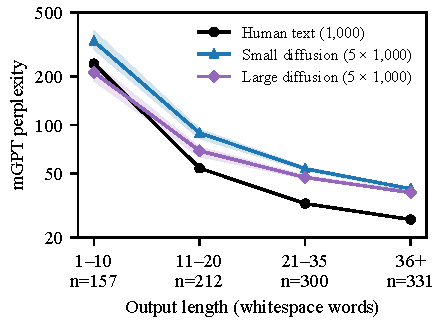
\includegraphics[width=\columnwidth]{figures/length_bands.pdf}
\caption{mGPT perplexity by output length on the test split, log scale: 1,000 human passages (counts per band under each label) and five runs of 1,000 outputs per diffusion size (line: mean of run values; shading: range). AR is omitted because it was evaluated on validation only.}
\label{fig:length}
\end{figure}

\paragraph{AR comparison and the decoder alone.} On 256 validation samples the ratios to AR are 0.6458 and 0.6087, well within 1.20. Random latents decoded by the same decoder, however, score 57.60 on the same 256 rows and 50.36 on all 1,000, about as well as small diffusion, so mGPT perplexity alone does not show what the denoiser adds. Human test text scores 33.62, but the scorer is strongly length-dependent: human passages of 1--10 words score 240.83 and those of 36+ words 25.93. Both diffusion sizes have higher perplexity than human text in every band longer than ten words (Figure~\ref{fig:length}). We also resampled the AR model under 18 temperature, top-$p$ and constraint settings to look for a better-matched comparator: six settings matched the least diverse diffusion run on distinct-2 and entropy, but every setting produced 36 to 112 exact training copies per 1,000 validation outputs, against at most 13 for any diffusion run on the same split, so none met the pre-set eligibility rule and no tuned comparison was made. The AR baseline is thus a bounded from-scratch comparator, not evidence that diffusion outperforms autoregression.

\subsection{Language, shared phrasing and a second scorer}
\label{sec:res-language}

\begin{table}[t]
\centering
\small
\setlength{\tabcolsep}{3pt}
\begin{adjustbox}{max width=\columnwidth}
\begin{tabular}{lccccc}
\toprule
& & Unrec. & 4-gram & \multicolumn{2}{c}{Std.\ PPL} \\
\cmidrule(lr){5-6}
Bank & Afrikaans & tokens & overlap & mGPT & Goldfish \\
\midrule
Human & 98.2 & 4.3 & 14.4 & -- & -- \\
Human, scored subset & 97.9 & 4.2 & 15.7 & 41.6 & 64.6 \\
Small diffusion & 96.3 & 5.8 & 8.7 & 71.3 & 194.3 \\
Large diffusion & 97.2 & 5.9 & 11.8 & 59.6 & 148.1 \\
AR, nucleus & 95.3 & 5.3 & 15.8 & 80.5 & 203.7 \\
Random latents & 5.5 & 70.5 & 0.0 & 107.6 & 98.4 \\
\bottomrule
\end{tabular}
\end{adjustbox}
\caption{Validation outputs (\%, except Std.\ PPL, the length-standardised perplexity). The 4,825-passage human pool was not scored by mGPT or Goldfish; scorer values are for an 811-passage human subset. Rows: 4,825 human passages; 5$\times$1,000 per diffusion size; 256 AR; 1,000 random latents. Unrec.: word tokens not in the \texttt{af\_ZA} dictionary. 4-gram overlap: share of word 4-grams found in the training split. Human intervals (document bootstrap): Afrikaans 96.5--98.7, unrecognised 3.2--5.7, overlap 10.2--19.4.}
\label{tab:language}
\end{table}

Most diffusion outputs are identified as Afrikaans, at rates near human text (Table~\ref{tab:language}); the small configuration falls just below the human interval, mostly in outputs of ten words or fewer. Unrecognised words are slightly more frequent than in human text. In an AI-assisted reading of 50 unrecognised words per group, 22 from diffusion were malformed against 8 from human text. Diffusion outputs share 8.7\% (small) and 11.8\% (large) of their word 4-grams with the training split, against 14.4\% for held-out human text. These checks describe the generated text; they do not link its errors causally to reconstruction errors.

The random-latent control shows why these checks matter. Its raw mGPT perplexity is close to diffusion's, yet only 5.5\% of its outputs are identified as Afrikaans. Length-standardised mGPT ranks it last, but Goldfish does not penalise it: its raw Goldfish perplexity is 56.1 against 159.4 and 133.5 for small and large diffusion, and even after standardisation Goldfish ranks it best (Table~\ref{tab:language}). Goldfish is therefore not a validated quality scorer for this use. For the named comparisons it agrees with mGPT in direction: the large-minus-small difference and the large configuration's advantage over AR are confirmed under both scorers (standardised ratios 0.84 and 0.74 under mGPT, 0.76 and 0.73 under Goldfish), but the small configuration's advantage over AR is not clear under either (mGPT 0.89 [0.76, 1.03]; Goldfish 0.95 [0.78, 1.16]). Two further checks failed their pre-set calibration and are not reported as results: MAUVE \citep{pillutla2021mauve} with LaBSE embeddings \citep{feng2022labse} scored two halves of human text at 0.14 against a required 0.90, and two local model judges missed the validation thresholds for applying the proposal's sample checklist.

\subsection{Interventions and full autoencoder training}
\label{sec:res-aescreen}

Three decoder changes, each with a threshold fixed in advance, were tried on the 81 passages: decoding without the trigram ban, and retraining the last two or all twelve decoder blocks. None passed. Retraining all twelve gave the largest gain, raising chrF from 67.70 to 70.05 (paired 95\% CI for the change [0.78, 3.96]) and numerals from 21 to 25 of 33, but stayed below the 70.70 chrF and 14-exact thresholds; its best checkpoint lay at the end of its budget.

\begin{table}[t]
\centering
\small
\begin{adjustbox}{max width=\columnwidth}
\begin{tabular}{llcccc}
\toprule
Arm & Data & Slots & Exact & chrF & Numerals \\
\midrule
Original & NCHLT & 32 & 26 & 69.24 & 0.62 \\
A & NCHLT & 32 & 118 & 96.35 & 0.94 \\
B & NCHLT & 64 & 126 & 97.89 & 1.00 \\
C & + extra & 32 & 121 & 96.51 & 0.99 \\
D & + extra & 64 & 134 & 98.20 & 1.00 \\
\midrule
\multicolumn{6}{l}{Reserve, 103 passages} \\
Original & NCHLT & 32 & 19 & 68.32 & 0.77 \\
D (winner) & + extra & 64 & 73 & 98.70 & 1.00 \\
\bottomrule
\end{tabular}
\end{adjustbox}
\caption{Autoencoder screen. Exact: exact reconstructions, out of 194 (comparison panel) or 103 (reserve). Numerals: recall of source numerals (a fraction, unlike the counts in Table~\ref{tab:recon}). + extra: NCHLT plus 511,155 words of other government-domain Afrikaans. Arms A--D train every parameter; the original trains only part of the model. Every arm stopped at its six-hour cap after about 3,500 of 10,000 planned updates.}
\label{tab:aescreen}
\end{table}

We then trained four new autoencoders under a protocol fixed before training (Table~\ref{tab:aescreen}), all following the full mT5-base recipe of \citet{lovelace2023latent}, with every parameter trained. The arms cross training data (NCHLT alone, or with 511,155 further words of deduplicated government-domain Afrikaans) with latent length (32 or 64 slots). Validation documents were divided into three disjoint panels: a 663-passage selection panel (whose documents also supply the 81 development passages), a 194-passage comparison panel and 103 reserve passages held back since 22 October. Arms were ranked on the selection panel, and the winner was evaluated once against the original on the reserve. Training all parameters at the original latent size raised exact matches on the comparison panel by 47.4 points (95\% CI [40.4, 54.7]); longer latents added 4 to 7 points, and extra data at most 4. The winner met all three reserve thresholds: 73 of 103 exact against 19 (difference 52.4 points, CI [42.5, 63.3]), chrF 98.70 against 68.32, and numeral recall 1.00 against 0.77. Exact matches on long reserve passages remain rare (1 of 15), although their chrF is 95.9. Diffusion on the new autoencoder was not complete for this version, so its effect on generation is not reported.

\subsection{A second language: Swahili}
\label{sec:swahili}
The Afrikaans checks changed how its perplexities had to be read: random latents matched diffusion on raw perplexity, and reconstruction, not the denoiser, limited fidelity. An earlier Swahili run of the same pipeline had been evaluated only by denoising loss and perplexity, the evaluation those checks showed to be insufficient, so we applied them to it without retraining. That run used two seeds per denoiser size and equal wall-clock budgets, so the small denoiser took about 172,000 updates and the large about 53,000; it has no AR baseline. Its test mGPT perplexity was 19.5 and 19.6 (small) and 20.6 and 20.8 (large), against 13.8 for human text. The checks followed a protocol approved before any model was run and used validation data only. Reconstruction of 200 passages reached mean chrF 74.8 (95\% CI [72.9, 76.5]) against 24.3 with shuffled latents, but no exact matches, and numeral recall was 0.54. Random latents decoded by the same decoder scored clearly worse (perplexity 135) than diffusion samples. GlotLID labelled all diffusion samples and references as Swahili, against 57\% of random-latent outputs. Diffusion outputs shared 10--11\% of their word 4-grams with the training split, against 28\% for references, which the supplied splits' cross-split overlap inflates. All readings are automatic and descriptive. The Afrikaans pattern recurs in a second language: fluent-scoring samples from a lossy autoencoder, which perplexity alone would not have revealed.

% ===========================================================================
\section{Discussion}
\label{sec:discussion}
% ===========================================================================

\paragraph{Verdict.} \emph{RQ1 is partly answered.} A reduced English control (ROCStories with BART, 5,000 updates) reached 93.26\% validation token accuracy and 11 of 128 exact reconstructions, so the training code runs and learns; this does not show adequate fidelity, and the English and Afrikaans rates come from different models and data. Shorter runs showed that very small batches fail and that BF16 at effective batch 16 can diverge. It cannot rule out faults specific to the Afrikaans mT5 configuration. \emph{RQ2's criterion is not met}: the original reconstructions change names, numerals and content words. The screen shows that this failure belongs to the original autoencoder, not to the setting. \emph{RQ3 is met only numerically.} The ratios are within 1.20 and diversity shows no collapse, but the comparison is unmatched and the scorer length-sensitive, so under the pre-specified rule it is a weak diagnostic; after length standardisation the small configuration's advantage is unclear. Fertility is reported descriptively (1.933 tokens per word). \emph{The hypothesis is not supported}, because credibility required adequate reconstruction.

\paragraph{Why scores and fidelity diverge.} Every sample passes through the same pretrained decoder with beam search, and both decoder and scorer were pretrained on large multilingual corpora that include Afrikaans (mT5 on mC4; mGPT on Wikipedia and C4). Random latents reach diffusion-level raw perplexity through this decoder, while reconstructions score 70.67 against 61.76 for their sources, so the decoder does not simply pull text towards high-probability Afrikaans. Raw perplexity therefore cannot separate what the denoiser contributes from what the decoder contributes, and it does not detect output that is not Afrikaans. A better denoiser changes which latents reach the decoder but cannot restore what the autoencoder fails to preserve. The failure lies in the encode--decode path; our measurements do not separate information missing from the latent from information the decoder fails to recover. We do not claim that it makes the generated text worse, which would need generation from the repaired autoencoder.

\paragraph{Under-adaptation or bottleneck?} We call an autoencoder under-adapted when its trainable parameters have not been trained enough to use the latent it has; a bottleneck is a latent too small to hold the passage, and predicts errors that grow with length and gains from a longer latent. On the reserve passages the original reconstructs 16 of 47 short, 3 of 41 medium and 0 of 15 long passages exactly, against 45, 27 and 1 for arm D; arm D's long-passage chrF is 95.9, high surface similarity despite few exact matches; whether their content is preserved is unverified. Training every parameter added 47 points of exact match, and longer latents 4 to 7. The new recipe also changes the batch size (128 against eight) and the training schedule, so the gain cannot be attributed to unfreezing alone, but the evidence favours under-adaptation of the original autoencoder over a fixed bottleneck.

% ===========================================================================
\section{Limitations and deviations}
\label{sec:limitations}
% ===========================================================================

The study covers one administrative corpus, one language (Swahili is checked descriptively only) and one task, and training text was not screened with language identification. The diffusion system inherits mT5 pretraining and the AR baseline does not; they also differ in decoding and compute, and the AR budget was set provisionally against an earlier diffusion run, so differences cannot be attributed to diffusion versus autoregression. mGPT perplexity is length-dependent, chrF and numeral matching are surface measures, and low repetition is partly enforced by decoding. Seeds are conditional on one autoencoder and one AR run, intervention gains are exploratory, and the test set is not untouched. Training rescales the self-conditioning estimate but sampling does not; its effect was not tested.

Departures from the proposal: the English control used ROCStories with BART, the supported upstream route, as a reduced implementation check rather than the proposed OpenWebText reproduction; the tokeniser is mT5's rather than a new SentencePiece vocabulary; the AR baseline matches corpus and tokeniser only; and the planned researcher checklists for reconstructions and samples were not completed, with no reason documented. There was no participant-based evaluation, as planned; reconstruction and sample readings were AI-assisted and not verified by an Afrikaans reader. Additions not in the proposal are five seeds per configuration, the latent controls, the decoder interventions, the autoencoder screen and the Swahili checks.

% ===========================================================================
\section{Conclusion}
% ===========================================================================

Adapting latent diffusion to Afrikaans produced samples with lower raw perplexity than a small, historical autoregressive comparator, and lower again with a larger denoiser, from an autoencoder that does not reproduce its inputs faithfully. Random latents passed through the same decoder scored almost as well. Retraining the decoder alone did not reach its thresholds; training the whole autoencoder substantially improved reconstruction on passages held back for that test. Whether better reconstruction yields better generation remains to be measured. For latent text diffusion in a new language, reconstruction fidelity should be measured and reported before generation scores are interpreted.

\section*{Statements}
\textbf{AI use.} AI assistance supported artifact auditing, analysis, sample and reconstruction inspection, drafting and LaTeX preparation; AI-assisted inspection is not human evaluation, and the author is responsible for the claims. \textbf{Ethics.} The corpus is publicly licensed and contact details were masked; no human participants were involved, and institutional ethics approval or exemption has not been verified. \textbf{Data and code.} Code, protocols and documentation: \url{https://github.com/hadibutt3560/afrikaans-latent-diffusion}; \texttt{REPRODUCIBILITY.md} at the repository root indexes the training configurations, scorer revisions, length-standardisation weights and band-support rule, and the interval procedures. Model weights, corpora and full sample banks are local artifacts not in the repository.

\bibliographystyle{acl_natbib}
\bibliography{references}

\end{document}
